% !TeX program = pdflatex
% !TeX spellcheck = en_US
% !TeX encoding = UTF-8

% update
% v.1.2 - 2018-10-15
% - Felix: use Bibtex instead of Biblatex
% v1.10 - 2017-05-30
% - Erik: Refactor the file structure of the front pages
% - Erik: Fix double bibliography entry
% v1.9 - 2017-02-03
% - Dirk: fixed warning: Underfull \hbox (badness 10000) in paragraph main.tex
% - Dirk: fixed warning: "Data encoding is UTF8" -> style.tex 0.1.8
% v1.8 - 2017-02-02
% - Dirk: replaced titlesec package by KOMA-script commands.-> style.tex v0.1.7
% v1.7 - 2014-11-18
% - bib fixes: now using biber instead of bibtex (thanks felix)
% - compile now with pdflatex -> biber -> pdflatex
% v1.6 - 2013-05-13
% - bibliography headers fixed - thanx lorenz lehmann
% - high quality titlepage - thanx thomas graf
% - removed separation of online and offline references -> style 1.4a
% v1.5 - 2013-01-16

\documentclass[twoside,11pt,titlepage,a4paper,english,bibliography=totocnumbered,listof=numbered]{scrbook}
%
% Template Style
% =========================================================================
% = SNET THESIS TEMPLATE STYLE
% =========================================================================

% http://www.snet.tu-berlin.de
% ------------------------
% Adapted version from http://hci.rwth-aachen.de/karrer_thesistemplate (Thorsten Karrer)
% Further adaptions for http://www.elearn.rwth-aachen.de (Sascha Hoellger)
% Further adaptions for SNET @ TU Berlin by Sebastian Göndör (sebastian.goendoer@tu-berlin.de)


% =========================================================================
% = CHANGELOG
% =========================================================================
% [0.1.9]
% - Fixed styling for chapters and toc using Komascript
% - Remove double bibliography TOC entry
%
% [0.1.8]
% - fixed "warning UFT8 is used". biblatex requires ascii encoding; by Dirk
%
% [0.1.7]
% replaced "Titelsec" commands (and whole package) by appropriate KOMA-Script commands; by Dirk
%
% [0.1.6]
% replaced deprecated \rm commands with \rmfamily commands; by Dirk
%
% [0.1.4b]
% backend=biber added in line 139
%
% [0.1.4a]
% title page: image logo sizes and margins adjusted to printable area
% removed separation of online and offline references
%
% [0.1.3]
% wider text body
% added "school" to the titlepage
% paragraph indents
% correctly placed footnote graphics
%
% [0.1.2]
% new titlepage
% some minor fixes
%
% [0.1.1]
% changed titlepage logo
% added listoffigures and listoftables
% excluded abstract from toc
% no (roman) numbering for frontmatter
%
% [0.1]
% adapted version 0.991b from sascha hoellger @ rwth aachen


% =========================================================================
% = MISC
% =========================================================================

\usepackage{a4wide}					%
\usepackage{verbatim}				%
\usepackage[toc,page]{appendix}			%
\usepackage[withpage]{acronym}			%
\usepackage{amsthm}				% Definitions


% =========================================================================
% = COLORS
% =========================================================================

%%%\usepackage{xcolor}			% Colors

\usepackage[table]{xcolor}
%%%\setlength{\arrayrulewidth}{1mm} table border Fontsize
\setlength{\tabcolsep}{18pt}
\renewcommand{\arraystretch}{1.8}
\newcolumntype{s}{>{\columncolor[HTML]{23a5e2}} p{3cm}}
 
\definecolor{LightBlue}{rgb}{0.55,0.55,1}
\definecolor{DarkBlue}{rgb}{0.2,0.2,0.5}
\definecolor{DarkRed}{rgb}{0.71,0.12,0.07}

% =========================================================================
% = PAGE LAYOUT
% =========================================================================

\usepackage{geometry}
\geometry{inner=3cm, outer=2cm, bottom=4cm}

\newcommand{\setwidesite}				% changes the geometry to have less margin
{
	\fancyhfoffset[LE,RO]{0cm}
	\fancyheadoffset[LO,RE]{0cm}
	\fancyfootoffset[RE]{2cm}
	\newgeometry{inner=2cm, outer=2cm, bottom=4cm}
}

\usepackage{style/noindent}				%do not indent at new paragraphs but add a vertical offset

\setlength{\parindent}{4mm}
\setlength{\parskip}{1.5mm }

%Line spacing
\renewcommand{\baselinestretch}{1.5}

% =========================================================================
% = TYPESETTING
% =========================================================================

\usepackage[hyphens]{url}				% url
\usepackage{hyphenat}				% hyphenation. use \hyphenation{}

\righthyphenmin=5
\lefthyphenmin=5


% =========================================================================
% = TABLE OF CONTENTS
% =========================================================================

\setcounter{secnumdepth}{4}
\setcounter{tocdepth}{3}

\addtokomafont{disposition}{\rmfamily}


% =========================================================================
% = FONTS
% =========================================================================

\usepackage{mathpazo}
\usepackage[scaled=.95]{helvet}
\usepackage{courier}


% =========================================================================
% = SYMBOLS
% =========================================================================

%\usepackage{gensymb}
\usepackage{textcomp} 				% for \textmu (non-italic $\mu$)
\makeatletter						% this makes "@" a regular letter


% =========================================================================
% = TABLES
% =========================================================================

\usepackage{tabularx}
\usepackage{booktabs}
\usepackage{multirow}
\usepackage{longtable}				% tables spanning over more than one page

%%\setlength{\fboxsep}{0mm}			% spacing between \fbox border and content

\usepackage{amsmath}				% math fonts
\usepackage{amssymb}				% math symbols
\usepackage{setspace}				% line spacing


% =========================================================================
% = BIBILOGRAPHY
% =========================================================================

% 2018-10-16 - changed to use Bibtex instead

%\usepackage[style=numeric,natbib=true,backend=biber]{biblatex}

% apparently no effect?
%\renewcommand{\bibsetup}{
%	\markboth{
%		\MakeUppercase{Bibliography}
%	}{}
%}

%\ifdefined\bibheadingonline
%  \defbibheading{online}{\section*{\bibheadingonline}}
%\else
%  \defbibheading{online}{\section*{Online References}}
%\fi
%\ifdefined\bibheadingoffline
%  \defbibheading{offline}{\section*{\bibheadingoffline}}
%\else
%  \defbibheading{offline}{\section*{Printed References}}
%\fi
%
%\defbibfilter{online}{%
%  \( \type{online} \)}
%
%\defbibfilter{offline}{%
%  \( \not \type{online} \)}
%
%\bibliography{Bibliography}


% =========================================================================
% = LANGUAGE & ENCODING
% =========================================================================

\usepackage[english]{babel}				 
%\usepackage[ngerman]{babel}

\selectlanguage{english}
%\selectlanguage{ngerman}

\usepackage[T1]{fontenc}
\usepackage[utf8]{inputenc}				% can use native umlauts

% \usepackage[babel,german=quotes]{csquotes}	% provides \enquote{Blupp} => "`Blupp"'
\usepackage[babel,english=american]{csquotes}	% provides \enquote{Blupp} => "`Blupp"'

%\SetCiteCommand{\parencite}			% Changed for biblatex

\usepackage{units}					% unified way of setting values with units

\usepackage{appendix}


% =========================================================================
% = CODE LISTINGS
% =========================================================================

\usepackage{listings}

% Listings Styles from Max

\definecolor{violet}{cmyk}{0.45,0.97,0.27,0.21}
\definecolor{lstblue}{cmyk}{1,0.80,0,0}
\definecolor{lstgreen}{cmyk}{0.71,0.21,0.65,0.22}
\definecolor{bluegrey}{cmyk}{0.56,0.24,0.11,0.05}
\definecolor{javadoc}{cmyk}{0.88,0.59,0,0}
\definecolor{lstgrey}{cmyk}{0.55,0.44,0.42,0.32}

\lstdefinelanguage{SQL}{
     keywords={},
     keywordstyle=\color{bluegrey}\bfseries,
     morekeywords=[2]{CREATE,TABLE,IF,NOT,EXISTS,NULL,SET,DEFAULT,PRIMARY,KEY,COLLATE,CHARACTER,AUTO_INCREMENT,ENGINE,CHARSET},
     keywordstyle={[2]\color{violet}\bfseries},
     otherkeywords={int,varchar,double,text,tinyint},
     sensitive=false,
     morecomment=[l][\color{lstgreen}]{//},
     morecomment=[s][\color{lstgreen}]{/*}{*/},
     morecomment=[s][\color{javadoc}]{/**}{*/},
     morestring=[b]',
     morestring=[b]"
  }
\lstdefinelanguage{PHP}{
     keywords={},
     keywordstyle=\color{bluegrey}\bfseries,
     morekeywords=[2]{static,function,if,return,pow,sin,cos,asin,min,sqrt,int},
     keywordstyle={[2]\color{violet}\bfseries},
     otherkeywords={@param, @returns, @author, @type, @link, @see},
     sensitive=false,
     morecomment=[l][\color{lstgreen}]{//},
     morecomment=[s][\color{lstgreen}]{/*}{*/},
     morecomment=[s][\color{javadoc}]{/**}{*/},
     morestring=[b]',
     morestring=[b]"
  }
\lstdefinelanguage{JavaScript}{
     keywords={},
     keywordstyle=\color{bluegrey}\bfseries,
     morekeywords=[2]{attributes, class, classend, do, empty, endif, endwhile, fail, function, functionend, if, implements, in, inherit, inout, not, of, operations, out, return, set, then, types, while, use},
     keywordstyle={[2]\color{violet}\bfseries},
     otherkeywords={@param, @returns, @author, @type, @link, @see},
     sensitive=false,
     morecomment=[l][\color{lstgreen}]{//},
     morecomment=[s][\color{lstgreen}]{/*}{*/},
     morecomment=[s][\color{javadoc}]{/**}{*/},
     morestring=[b]',
     morestring=[b]"
  }
\lstdefinelanguage{Java}{
     keywords={},
     keywordstyle=\color{bluegrey}\bfseries,
     morekeywords=[2]{abstract,boolean,break,byte,case,catch,char,class,
      const,continue,default,do,double,else,extends,false,final,
      finally,float,for,goto,if,implements,import,instanceof,int,
      interface,label,long,native,new,null,package,private,protected,
      public,return,short,static,super,switch,synchronized,this,throw,
      throws,transient,true,try,void,volatile,while},
     keywordstyle={[2]\color{violet}\bfseries},
     morekeywords=[3]{@SuppressWarnings, @Capability, @Override},
     keywordstyle={[3]\color{lstgrey}},
     otherkeywords={@param, @return, @returns, @author, @link, @see},
     sensitive,
     morecomment=[l]//,
     morecomment=[s]{/*}{*/},
     morecomment=[s][\color{javadoc}]{/**}{*/},
     morestring=[b]",
     morestring=[b]',
  }[keywords,comments,strings]

% some listings styles from Gregor Aisch
% http://vis4.net/blog/2009/09/noch-mehr-sprach-definitionen-fuer-latex-listings/

\lstdefinelanguage{HTML5} {morekeywords={a, abbr, address, area, article, aside, audio, b, base, bb, bdo, blockquote,  body, br, button, canvas, caption, cite, code, col, colgroup, command, datagrid, datalist, dd, del, details, dialog, dfn, div, dl, dt, em, embed, eventsource, fieldset, figure, footer,  form,  h1, h2,  h3,  h4, h5,  h6,  head,  header,  hr, html,  i, iframe,  img,  input,  ins, kbd,  label,  legend,  li,  link,  mark,  map,  menu,  meta,  meter,  nav,  noscript,  object,  ol,  optgroup,  option,  output,  p,  param,  pre,  progress,  q,  ruby,  rp,  rt,  samp,  script,  section,  select,  small,  source,  span,  strong,  style,  sub,  sup,  table,  tbody,  td,  textarea,  tfoot,  th,  thead,  time,  title,  tr,  ul,  var,  video},
sensitive=false, morecomment=[s]{<!--}{-->}, morestring=[b]", morestring=[d]'}

\lstdefinelanguage{CSS} {morekeywords={azimuth,  background-attachment,  background-color,  background-image,  background-position,  background-repeat,  background,  border-collapse,  border-color,  border-spacing,  border-style,  border-top, border-right, border-bottom, border-left,  border-top-color, border-right-color, border-bottom-color, border-left-color,  border-top-style, border-right-style, border-bottom-style, border-left-style,  border-top-width, border-right-width, border-bottom-width, border-left-width,  border-width,  border,  bottom,  caption-side,  clear,  clip,  color,  content,  counter-increment,  counter-reset,  cue-after,  cue-before,  cue,  cursor,  direction,  display,  elevation,  empty-cells,  float,  font-family,  font-size,  font-style,  font-variant,  font-weight,  font,  height,  left,  letter-spacing,  line-height,  list-style-image,  list-style-position,  list-style-type,  list-style,  margin-right, margin-left,  margin-top, margin-bottom,  margin,  max-height,  max-width,  min-height,  min-width,  orphans,  outline-color,  outline-style,  outline-width,  outline,  overflow,  padding-top, padding-right, padding-bottom, padding-left,  padding,  page-break-after,  page-break-before,  page-break-inside,  pause-after,  pause-before,  pause,  pitch-range,  pitch,  play-during,  position,  quotes,  richness,  right,  speak-header,  speak-numeral,  speak-punctuation,  speak,  speech-rate,  stress,  table-layout,  text-align,  text-decoration,  text-indent,  text-transform,  top,  unicode-bidi,  vertical-align,  visibility,  voice-family,  volume,  white-space,  widows,  width,  word-spacing,  z-index},
sensitive=false, morecomment=[s]{/*}{*/}, morestring=[b]", morestring=[d]'}

\lstdefinelanguage{JavaFX} {morekeywords={abstract, after, and, as, assert, at, attribute, before, bind, bound, break, catch, class, continue, def, delete, else, exclusive, extends, false, finally, first, for, from, function, if, import, indexof, in, init, insert, instanceof, into, inverse, last, lazy, mixin, mod, new, not, null, on, or, override, package, postinit, private, protected, public-init, public, public-read, replace, return, reverse, sizeof, static, step, super, then, this, throw, trigger, true, try, tween, typeof, var, where, while, with },
sensitive=false, morecomment=[l]{//}, morecomment=[s]{/*}{*/}, morestring=[b]", morestring=[d]'}

\lstdefinelanguage{MXML} {morekeywords={mx:Accordion, mx:Box, mx:Canvas, mx:ControlBar, mx:DividedBox, mx:Form, mx:FormHeading, mx:FormItem, mx:Grid, mx:GridItem, mx:GridRow, mx:HBox, mx:HDividedBox, mx:LinkBar, mx:Panel, mx:TabBar, mx:TabNavigator, mx:Tile, mx:TitleWindow, mx:VBox, mx:VDividedBox, mx:ViewStack, mx:Button, mx:CheckBox, mx:ComboBase, mx:ComboBox, mx:DataGrid, mx:DateChooser, mx:DateField, mx:HRule, mx:Image, mx:Label, mx:Link, mx:List, mx:Loader, mx:MediaController, mx:MediaDisplay, mx:MediaPlayback, mx:MenuBar, mx:NumericStepper, mx:ProgressBar, mx:RadioButton, mx:RadioButtonGroup, mx:Spacer, mx:Text, mx:TextArea, mx:TextInput, mx:Tree, mx:VRule, mx:VScrollBar, mx:Application, mx:Repeater, mx:UIComponent, mx:UIObject, mx:View, mx:FlexExtension, mx:UIComponentExtension, mx:UIObjectExtension, mx:Fade, mx:Move, mx:Parallel, mx:Pause, mx:Resize, mx:Sequence, mx:WipeDown, mx:WipeLeft, mx:WipeRight, mx:WipeUp, mx:Zoom, mx:EventDispatcher, mx:LowLevelEvents, mx:UIEventDispatcher, mx:CurrencyFormatter, mx:DateFormatter, mx:NumberFormatter, mx:PhoneFormatter, mx:ZipCodeFormatter, mx:CursorManager, mx:DepthManager, mx:DragManager, mx:FocusManager, mx:HistoryManager, mx:LayoutManager, mx:OverlappedWindows, mx:PopUpManager, mx:SystemManager, mx:TooltipManager, mx:CreditCardValidator, mx:DateValidator, mx:EmailValidator, mx:NumberValidator, mx:PhoneNumberValidator, mx:SocialSecurityValidator, mx:StringValidator, mx:ZipCodeValidator, mx:DownloadProgressBar, mx:ArrayUtil, mx:ClassUtil, mx:Delegate, mx:ObjectCopy, mx:URLUtil, mx:XMLUtil, mx:CSSSetStyle, mx:CSSStyleDeclaration, mx:CSSTextStyles, mx:StyleManager, mx:HTTPService, mx:RemoteObject, mx:Service},
sensitive=false, morecomment=[s]{<!--}{-->}, morestring=[b]", morestring=[d]'}

\lstdefinelanguage{LZX} {morekeywords={a, alert, animator, animatorgroup , attribute, audio , axis, axisstyle , b, barchart, basebutton , basebuttonrepeater , basecombobox , basecomponent , basedatacombobox , basedatepicker , basedatepickerday , basedatepickerweek , basefloatinglist , basefocusview , baseform , baseformitem , basegrid , basegridcolumn , baselist , baselistitem , basescrollarrow , basescrollbar , basescrollthumb , basescrolltrack , baseslider , basestyle , basetab , basetabelement , basetabpane , basetabs , basetabsbar , basetabscontent , basetabslider , basetrackgroup , basetree , basevaluecomponent , basewindow , br , button , canvas , chart , chartbgstyle , chartstyle , checkbox , class , columnchart , combobox , command , connection , connectiondatasource , constantboundslayout , constantlayout , datacolumn , datacombobox , datalabel , datamarker , datapath , datapointer , dataselectionmanager , dataseries , dataset , datasource , datastyle , datastylelist , datatip , datepicker , debug , dragstate , drawview , edittext , event , face , floatinglist , font , font , form , frame , grid , gridcolumn , gridtext , handler , hbox , horizontalaxis , hscrollbar , i , image , img , import , include , inputtext , javarpc , label , labelstyle , layout , legend , library , linechart , linestyle , list , listitem , LzTextFormat , menu , menubar , menuitem , menuseparator , method , modaldialog , multistatebutton , node , p , param , piechart , piechartplotarea , plainfloatinglist , plotstyle , pointstyle , pre , radiobutton , radiogroup , rectangularchart , regionstyle , remotecall , resizelayout , resizestate , resource , reverselayout , richinputtext , rpc , script , scrollbar , security , selectionmanager , sessionrpc , simpleboundslayout , simpleinputtext , simplelayout , slider , soap , splash , stableborderlayout , state , statictext , style , submit , swatchview , SyncTester , tab , tabelement , tabpane , tabs , tabsbar , tabscontent , tabslider , Test , TestCase , TestResult , TestSuite , text , textlistitem , tickstyle , tree , u , valueline , valuelinestyle , valuepoints , valuepointstyle , valueregion , valueregionstyle , vbox , verticalaxis , view , view , vscrollbar , webapprpc , window , windowpanel , wrappinglayout , XMLHttpRequest , xmlrpc , zoomarea},
sensitive=false, morecomment=[s]{<!--}{-->}, morestring=[b]", morestring=[d]'}

\lstset{
  numbers=left,
  numberstyle=\tiny,
  numbersep=5pt,
  breaklines=true,
  stepnumber=1,
  tabsize=2,
  basicstyle=\ttfamily\small,
  frame=none,
  numberfirstline=true,
  firstnumber=1,
  keywordstyle=\color{violet}\bfseries,
  ndkeywordstyle=\color{bluegrey}\bfseries,
  identifierstyle=\color{black},
  commentstyle=\color{lstgreen}\ttfamily,
  stringstyle=\color{lstblue}\ttfamily,
  showstringspaces=false
}


% ========================================================================
% = CHANGE LIST DEFINITIONS
% ========================================================================

% change color of item list
\renewcommand{\labelitemi}{\color{black}$\bullet$}
\renewcommand{\labelitemii}{\color{black}$\circ$}
\renewcommand{\labelitemiii}{\color{black}$\ast$}
\renewcommand{\labelitemiv}{\color{black}$\diamond$}

% change color of enum list
\renewcommand{\labelenumi}{\color{black}\arabic{enumi}.}
\renewcommand{\labelenumii}{\color{black}\alph{enumii})}
\renewcommand{\labelenumiii}{\color{black}\roman{enumiii}.}
\renewcommand{\labelenumiv}{\color{black}\Alph{enumiv}.}

% change color of description list
\usepackage{enumitem}
\setdescription{font=\color{black}\rmfamily\itshape}
% \renewenvironment{description}{\list{font=\color{DarkRed}\itshape}}{\endlist}


% ========================================================================
% = FOOTNOTES
% ========================================================================

% change color of footnotes
\renewcommand{\thefootnote}{\color{black}\arabic{footnote}}

% use nice footnote indentation
\deffootnote[1em]{1em}{1em}{\textsuperscript{\thefootnotemark}\,}


% =========================================================================
% = GRAPHICS AND IMAGES
% =========================================================================

\usepackage{graphicx}
\graphicspath{{images/}}				% path to your image folder

\usepackage{eso-pic}					% needed for the full-face titlepage
\usepackage{chngpage}				% we need this to determine if a figure is on an odd or even page
\usepackage{tikz}					% tikz pictures

% captions of tables and images
\usepackage[hang,small,sf]{caption}
\renewcommand{\captionfont}{\sffamily\small}
\renewcommand{\captionlabelfont}{\bfseries}

\usepackage{float}
\usepackage{placeins}
% \floatstyle{ruled}
%\floatplacement

\renewcommand{\floatpagefraction}{0.85}		% if a figure takes more than 85% of a page it will be typeset on a separate page
\usepackage[it,bf,tight,hang,raggedright]{subfigure}

%\numberwithin{figure}{section}
%\numberwithin{table}{section}


% =========================================================================
% = HEADER
% =========================================================================

\newcommand{\STYLEfootnotetext}
{
  \begin{minipage}
  {.2\textwidth}
   
  \end{minipage}
}

% Change page headers and footers:
\usepackage{calc}
\usepackage{fancyhdr}
\pagestyle{fancy}
\fancyhfoffset[RO,LE]{0.1cm} %{\marginparsep+\marginparwidth}
\fancyhfoffset[RE,LO]{0.1cm}
%\fancyheadoffset[RE,LO]{\hoffset + \oddsidemargin}
\renewcommand{\headrule}{{\color{black}%
  \hrule width\headwidth height\headrulewidth \vskip-\headrulewidth}}
\fancyhf{}
\fancyhead[RE]{\slshape \nouppercase{\leftmark}}    % Even page header: "page   chapter"
\fancyhead[LO]{\slshape \nouppercase{\rightmark}}   % Odd  page header: "section   page"
\fancyhead[RO,LE]{\bfseries \thepage}

%- \fancyfoot[LE]{\STYLEleftpicture}
%- \fancyfoot[RO]{\STYLErightpicture}
\fancyfoot[LE]{\STYLEfootnotetext}

\renewcommand{\headrulewidth}{1pt}    % Underline headers
\renewcommand{\footrulewidth}{0pt}

% =========================================================================
% = SECTIONS THEMING
% =========================================================================

\newcommand{\allsectionformat}{\color{black}\rmfamily\normalfont}

% Font style and colors
\addtokomafont{part}{\Huge\allsectionformat}
\addtokomafont{chapter}{\Huge\allsectionformat}
\addtokomafont{section}{\allsectionformat}
\addtokomafont{subsection}{\allsectionformat}
\addtokomafont{subsubsection}{\allsectionformat}
\addtokomafont{paragraph}{\allsectionformat}
\addtokomafont{subparagraph}{\allsectionformat}

% Spacing before and after the section titles
\RedeclareSectionCommand[
  beforeskip=-.75\baselineskip,
  afterskip=.5\baselineskip]{section}

\RedeclareSectionCommand[
  beforeskip=-5\baselineskip,
  afterskip=.5\baselineskip]{chapter}


% =========================================================================
% = TYPESETTING - TWEAKES
% =========================================================================

\addtokomafont{section}{\LARGE}
\addtokomafont{subsection}{\large}

% instead of sloppy
%\tolerance 1414
%\hbadness 1414
%- \tolerance 2414
%- \hbadness 2414
%- \emergencystretch 1.5em
%- \hfuzz 0.3pt
%- \widowpenalty=10000     % Hurenkinde r
%- \clubpenalty=10000      % Schusterjungen
%- \brokenpenalty=10000
%- \interlinepenalty=9000 % seitenumbruch im absatz
%- \vfuzz \hfuzz
%- \raggedbottom


% =========================================================================
% =  USER DEFINED COMMANDS
% =========================================================================

\newcommand{\chapterquote}[2]{
    \begin{quotation}
    \begin{flushright}
    \noindent\emph{``{#1}''\\[1.5ex]---{#2}}
    \end{flushright}
    \end{quotation}
}


% custom hyphenation					% add words to this list to prevent hyphenation
\hyphenation{ ASCII TCP }

%make readable references

\usepackage{mathtools}% http://ctan.org/pkg/mathtools

 








\usepackage{CJKutf8}
\usepackage[acronym]{glossaries}
\usepackage[pdftex,pdfpagelabels=true]{hyperref}
\hypersetup{%
	pdftitle={Thesis Title},
	pdfauthor={Thesis Author},
	pdfkeywords={key1, key2, key3},
	pdfsubject={Thesis Subject}
}

% Adding a finite stretch on the page suppresses "Underfull \vbox (badness 10000)" warnings.
\makeatletter
\def\@textbottom{\vskip \z@ \@plus 1pt}
\let\@texttop\relax
\makeglossaries
\makeatother



\begin{document}


%--------------------------------------------------------------
% FRONT PAGE AND DOCUMENT METADATA
%--------------------------------------------------------------
\frontmatter

\begin{titlepage}
	\AddToShipoutPicture*{
		\put(0,0){

		}
	}
	\strut
	\hfill
	\begin{center}
	\vspace{0.5cm}
		\Huge
		\begin{spacing}{.9}
			\textcolor{black}{\textbf{Accented Speech Recognition}}\\
		\end{spacing}
		\vspace{0.8cm}
		\large
		by\\
		\vspace{0.8cm}
		\textbf{Mohamed Mesto}\\
		\vspace{0.8cm}
		\textbf{Matriculation Number 390***}\\
			\vspace{0.8cm}
		
\includegraphics[width=0.2 \textwidth]{images/TUBerlin.png}\\
	 	A thesis submitted to\\
		\vspace{0.8cm}
		Technische Universität Berlin\\
		Faculty IV - Electrical Engineering and Computer Science\\
		Institut für Softwaretechnik und Theoretische Informatik\\
		Quality and Usability Lab\\
		\vspace{0.5cm}
		Master's / Bachelot's Thesis\\
		\vspace{1cm}
		\today\\
		\large
		Supervised by:\\
		Prof. Dr. Sebastian Möller \\
		Dr. Tim Polzehl \\
		\end{center}

\end{titlepage}



\chapter*{\LARGE Eidestattliche Erklärung / Statutory Declaration}
Hiermit erkläre ich, dass ich die vorliegende Arbeit selbstständig und eigenhändig sowie ohne unerlaubte fremde Hilfe und ausschließlich unter Verwendung der aufgeführten Quellen und Hilfsmittel angefertigt habe.
\vspace{2em}

\noindent I hereby declare that the thesis submitted is my own, unaided work, completed without any unpermitted external help. Only the sources and resources listed were used.

The independent and unaided completion of the thesis is affirmed by affidavit:

\vspace{30 mm}
\begin{flushright}

\rule{90mm}{1pt}

Berlin, \today \hspace{15 mm} Name 
\end{flushright}

\chapter*{Acknowledgments}
\label{cha:acknowledgments}

First of all, I would like to thank .... 
    

\chapter*{Abstract}
\label{cha:abstract}

My Abstract ....


			% EN Abstract
\chapter*{Zusammenfassung}
\label{cha:zusammenfassung}

summary in GERMAN



	% DE Abstract

\tableofcontents{}
% Lists of tables and figures
\listoffigures
\listoftables


%--------------------------------------------------------------
% MAIN CONTENT
%--------------------------------------------------------------
\mainmatter

%\part{}						% optional: use parts to structure your thesis



\chapter{Introduction}
\label{cha:introduction}
\section{Motivation}

In this paper, we will address the main engine in the field of neural networks\cite{dai2019transformer,devlin2018bert,raffel2020exploring} in general and automatic speech recognition in particular, which is transformers\cite{vaswani2017attention}. What contributed to her gaining this reputation is the multi-head self-attention approach, which instantly provides a high-handed position connection in parallel for the entire series, Instead of utilizing memory conditions to catch long-range dependencies in recurrent neural networks.

Nevertheless, the noteworthy transformer-based model architectures in automatic speech recognition (ASR) are Connectionist temporal classification (CTC)\cite{salazar2019self,zhang2020faster},
sequence-to- sequence \cite{dong2018speech,karita2019comparative,sperber2018self,zhou2018syllable,wang2020low}, Neural transducer \cite{zhang2020transformer,yeh2019transformer,gulati2020conformer} and traditional hybrid systems\cite{wang2020transformer,povey2018time}.


The results of the tests carried out on the public LibriSpeech showed a resounding success. The Emformer achieved a very low Word Error Rate (WER) in the clean-up test for a certain average latency \cite{shi2021emformer}. Nevertheless, One of the promising technologies in this field is the Transformer Transducer. It exceeded the neural transducer with the Long-Short Term Memory (LSTM) or the Bidirectional Long-Short Term Memory (BLSTM) networks and achieved a surprising WER on the test-clean set and the test-other set.\cite{yeh2019transformer}. Moreover, One of the new technologies that grabbed the spotlight was the wav2vec2 pretrained model. It supported the ASR Systems in the Dysarthric speech recognition field\cite{karthick2022speaker}. 


\subsection{Improved/significantly improved}
\section{Background}
text .... Wikipedia \footnote{https://www.wikipedia.org/}




\section{Problem Statement}

 

\section{Outline}


\chapter{Literature Review}
\label{cha:relatedwork}




\section{Speech Recognition}


During the last decades, the reliability of the speech recognition system has increased and its use in solving many industrial, medical and various challenges in different areas of daily life\cite{benesty2008automatic}.
Automatic Speech Recognition (ASR), computer speech recognition, or Speech-To-Text (STT) are all terms for the concept of speech recognition. It is a sub-domain of the joint work between computer science, computer engineering, and computational linguistics. His work is summarized by approaches and procedures that allow the recognition of spoken language and its translation into text by computers\footnote{https://www.wikipedia.org/}.
In this paper, we will discuss some of these techniques, the most important of which are: Emformer Model \cite{shi2021emformer,dai2019transformer}, DeepSpeech Model \cite{markert21_spsc}, Wav2vec2 \cite{karthick2022speaker}, Transformer-Transducers \cite{yeh2019transformer}, Conformer Model \cite{gulati2020conformer}, Recurrent Neural Network Transducer (RNN-T)\cite{zhang2020transformer}, and others. The following is a brief intro to each method as well as its advantages and disadvantages.

\section{Acoustic Models}
\subsection{Non-streaming versus Streaming Models}

Audio formats performed through the Web fall into two general classifications. The user must download non-streaming audio files to the user's hard disk before being able to play after that, unlike Streaming audio files, which can play almost immediately and continue playing while they are downloading. However, each category has advantages and disadvantages. In artificial intelligence algorithms specialized in dealing with linguistics, stream processing is a programming layout that considers data streams, or series of events in time, as the primary input and output entities of analysis. Parallel computing empowers the Stream processing systems for data streams and relies on streaming algorithms for efficient performance\footnote{https://www.wikipedia.org/}.

 
 An additional detailed discussion of specific streaming and non-streaming acoustic models follows.




\subsection{AM-TRF Model}
The Streaming Transformer with Augmented Memory (AM-TRF) \cite{wu2020streaming} ...

\textbf{\ref{fig:AM-TR-Emformer}a}

 



\subsection{Emformer Model }
%\subsubsection{Motivation}
Efficient Memory transformer based acoustic model for low latency streaming speech recognition is referred to simply as Emformer. It is one of the promising technologies in Accented Speech Recognition field. It earns this position because of the enhancement of the AM-TRF model. First, Emformer reduces the enumeration by extracting the repeated calculation from the left context block by caching the key and value in earlier segments' self-attention. Second, Emformer carries over the memory bank from the lower layer instead of passing the memory bank within the recent layer in AM-TRF motivated from the Transformer-XL features \cite{dai2019transformer, lu2020exploring}. Third, Emformer stops the resume vector's attention with the memory bank to evade overweighting the most left element of context information. Finally, the significant property of the Emformer for low latency speech recognition is presented in a parallelized block processing training strategy \cite{shi2021emformer}.

%\subsubsection{Emformer Mechanism}

As shown in the previous paragraph, though, the AM-TRF has proven itself in the field of Accented Speech Recognition\cite{wu2020streaming}. But his performance in the left context was unsatisfactory. Moreover, The main impetus behind the development of the Emformer technology is due to the shortcomings in implementing concatenated processing by AM-TRF.  Figure \textbf{\ref{fig:AM-TR-Emformer}b} shows one layer of the Emformer. The following subsections represent the significant advancements completed in Emformer.

\begin{figure}[!ht]
	\centering
	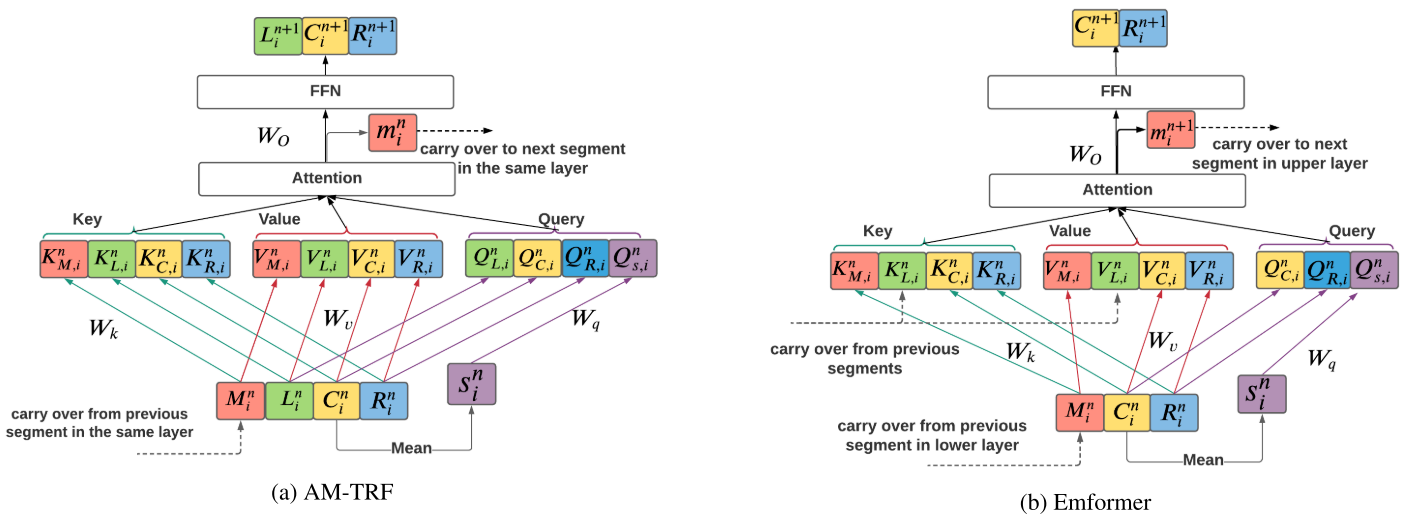
\includegraphics[width=1 \textwidth]{images/AM-TR-Emformer.png}\\
	\caption{Comparison of AM-TRF with Emformer overlapping}
    \caption*{\cite{shi2021emformer}}
	\label{fig:AM-TR-Emformer}
\end{figure}






\begin{itemize}
    \item Cache key and value from previous segments
 


In the AM-TRF model, Figure \textbf{\ref{fig:AM-TR-Emformer}a} , the re-computation of \( L_{i}^{n}\) for every step is required during the processing. Hence we need only to cache the projections from the earlier segments. The improvements of the Emformer are displayed in Figure \textbf{\ref{fig:AM-TR-Emformer}b}. There is only demand to compute the key, and value projections for the memory bank, center, and right context. Besides, Since there is no need to give output from the left context block for the next layer, Emformer holds the computation of query projection of the left context.

 To understand the superiority of the Emformer over the AM-TRF, we will assume the following:\\
M: is the length of the memory bank. \\
L: is the length of the left context block.\\ 
R: is the length of the right context.\\ 
C: is the length of the center context. \\
h: is the number of heads in the multi-head self-attention, and per head dimension is d. \\
Besides, the mean of the center segment That takes the value one is equal to the summary vector \( S_{i}^{n}\). Nevertheless, the model dimension, dh, is substantially more enormous than any of M, L, R, and C. The implementation of the memory bank utilizes a ring buffer form with a short length. Hence, the Emfromer is more efficient than the AM-TRF by keeping around \(  \frac{L}{L+R+C}\)  of AM-TRF computation \cite{shi2021emformer}.


 
 \item Carryover Memory Vector from Earlier Segments in the Lower Layer




To benefit from the opportunities proposed by the Graphics processing unit (GPU), Emformer supports block processing in parallel during the training stage. It takes the memory bank input from previous segments in the lower layer instead of the same layer. Accordingly, the whole sequence is trained in parallel for each Emformer layer \cite{shi2021emformer}. Unlikely to the AM-TRF Method. Whereas the auto-regression feature causes the block processing to be sequential.
 
 \item Prevent Attention between the Summary Vector with the Memory Bank

To avoid the gradient disappearance or damage in the Emformer Technology. Moreover, to achieve a stable training accuracy for long-form speech, we need to allocate the attention weight between the summary vector and the memory bank to zero. At odds, embedding the memory bank information in the recent memory vector amplifies the most left context information \cite{shi2021emformer}.  


 \item Look-Ahead Context Leaking handling

During the training scenario, Emformer handles the input sequence quite parallel. Instead of physically dividing the input sequence into each layer, Emformer involves attention masks to limit the reception field \cite{dai2019transformer,chen2021developing}. Unfortunately, this method has disadvantages represented in the look-ahead of context leaking. Adding to the actual size of the right context is when multiple transformer layers are stacked on top of each other. The right side of
 Figure \textbf{\ref{fig:Avoiding-look-ahead-context-leaking}} shows how the Emformer avoids the look-ahead context leaking case during the training process. Emformer produces a hard copy of each segment's look-ahead context and sets the look-ahead context copy at the input sequence's start. To understand the concept, as we notice, the output in frame 5 in the first chunk only uses the information from the current piece jointly with frame 8 of the right context, excluding the right context leaking.

 

 

\begin{figure}[!ht]
	\centering
	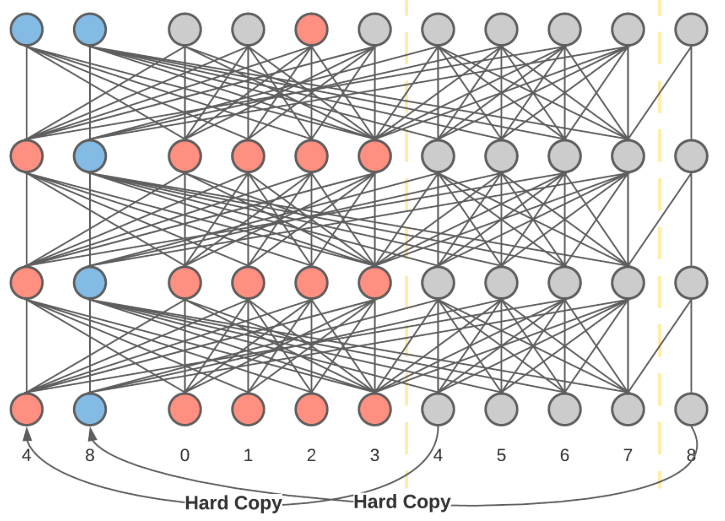
\includegraphics[width=0.8 \textwidth]{images/Avoiding-look-ahead-context-leaking.png}\\
	\caption{ Representative of preventing look-ahead context leaking. Considering that:\\
	The chunk size value is 4, and the right context size is 1}
    \caption*{\cite{shi2021emformer}}
	\label{fig:Avoiding-look-ahead-context-leaking}
\end{figure}


\end{itemize}




\subsection{Deepspeech Model}


%\subsubsection{Motivation}

 
Alongside human life development, ASR systems' challenges are becoming very high due to the complicated architecture of deep neural networks (DNNs). Moreover, information systems that depend on audio inputs have integrated all the service devices surrounding us. Including IoT and personal identification systems in the home, Alexa\footnote{https://developer.amazon.com/en-GB/alexa} has a built-in ASR to comprehend our instructions. In our cars like summalinguae\footnote{https://summalinguae.com/language-technology/the-present-and-future-of-in-car-speech-recognition/}, workplace ,or PCs (e.g., to speak with Cortana\footnote{https://www.microsoft.com/en-us/cortana/} virtual assistant in Windows PC). Furthermore, in our mobile devices, there are ASRs that we can use to type texts or communicate with a mobile virtual assistant (e.g., Siri\footnote{https://www.apple.com/siri/} and Google Assistant\footnote{https://assistant.google.com/}). Which increased the risks of manipulating them on the lives of individuals or societies to an unimaginable extent \cite{hu2019adversarial,abdullah2021sok}. These manipulated inputs are called audio adversarial examples. The goal of these procedures is to deliver audio inputs different from the natural inputs to break into the property of others, such as accessing and controlling the work system of a company, house, or car. This misconception may risk the privacy of people \cite{carlini2018audio,mitev2020leakypick}.

In this chapter, as a study use case, we will focus on, DeepSpeech, an End-to-End model for ASR. Furthermore, Deeply highlights a class of interpretability algorithms named attribution-based approaches \cite{ancona2017towards,sundararajan2017axiomatic}. This strategy aims to estimate the DNN's most significant input's attributions to the output's behavior. Hence, we handle three visualization techniques: Shapley Additive Explanations (SHAP), Layer-wise Relevance Propagation (LRP), and Saliency Maps. We compare these methods and discuss possible applications, such as detecting adversarial examples \cite{carlini2018audio, qin2019imperceptible, dorr2020towards}.



%\subsubsection{Deepspeech Mechanism}

 The input of the DeepSpeech function is digital audio to generate the output "considerable possible" text transcript of that audio. Which grant it the name "automatically transcribing spoken audio tool." \footnote{https://mozilla.github.io/deepspeech-playbook/}.

The mechanism of action of the DeepSpeech represented in 
taking a stream of audio as input and converting that stream of audio into a sequence of characters in the established alphabet \cite{asyrofi2020crossasr}. Since there are two phases to be implemented. The audio is converted into a series of possibilities over characters in the alphabet in the first stage. Secondly, this series of options is converted into a string of characters.
To achieve the first stage, we employ the Deep Neural Network. The DNN is trained on the audio and matchable text transcripts. Moreover, the neural model is qualified to predict the text from speech. Therefore, the first phase, the acoustic model, is well-deservedly called a phonetic transcriber. Besides, an N-gram language model is involved in accomplishing the second phase \cite{markert2022language,michel2019evaluation}. The N-gram language model is trained on a text collection that is usually various from the text transcripts of the audio. Furthermore, The language model is trained to predict text from the previous text. In other words, we can consider the language model as a spelling and grammar checker.

% \subsubsection{Layer-wise Relevance Propagation (LRP)}


% \subsubsection{Saliency Maps}

% \subsubsection{Shapley Additive Explanations (SHAP)}
 



% \subsubsection{Background on DeepExplain and DeepSpeech}


 \textbf{\ref{fig:Architecture-of-CrossASR}} 





\begin{figure}[!ht]
	\centering
	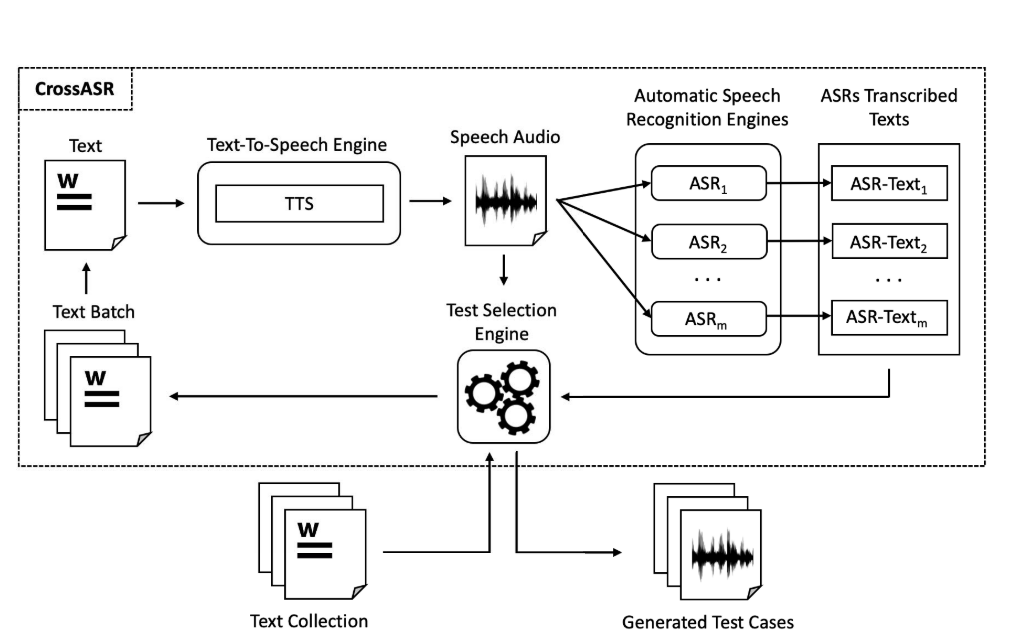
\includegraphics[width=0.8 \textwidth]{images/Architecture-of-CrossASR.png}\\
	\caption{Architecture of CrossASR}
    \caption*{\cite{asyrofi2020crossasr}}
	\label{fig:Architecture-of-CrossASR}
\end{figure}



\subsection{Wav2Vec2 Model}

\subsection{Conformer Model}
\subsection{RNN-T Model}
% \subsection{RIVA Model}

 



\section{Language Models}
\subsection{N-gram Model}
\subsection{Transformer Model}
\subsection{GPTx Model}


\section{Streaming/non-streaming Models}


\chapter{Data Augmentation}
\section{Data Augmentation - Noise Factor}
\section{Data Augmentation - Time Factor}
 

 

 



\chapter{Experimentation}
\label{cha:comparison}
\section{Dataset}


pip install seaborn

Python for Data Science and Machine Learning Bootcamp : Distribution Plots

https://www.youtube.com/watch?v=lTc7NU9XpWE

https://seaborn.pydata.org/installing.html

% https://www.w3schools.com/python/numpy/numpy_random_seaborn.asp

https://seaborn.pydata.org/tutorial/distributions.html



\section{Improved/ significantly improved}



Data Augmentation (noise, time) --> librosa, specAug






**************
That is what I would do as you could still introduce RTF, WER etc. in later sections and describe the results in better detail. 

Will refine again

*********

The results of the tests carried out on the public LibriSpeech showed a resounding success. The Emformer achieved a WER of 2.50\text{\%}in the clean-up test and 5.62\text{\%} in the other-test for an average latency of 960ms \cite{shi2021emformer}. Besides, at a low latency of 80 ms, Emformer gains WER 3.01\text{\%} on test-clean and 7.09\text{\%} on test-other. Nevertheless, One of the promising technologies in this field is the Transformer Transducer. It exceeded the neural transducer with LSTM/BLSTM networks and achieved a WER of 6.37\text{\%} on the test-clean set and 15.30\text{\%} on the test-other set\cite{yeh2019transformer}. Moreover, One of the new technologies that grabbed the spotlight was the wav2vec2 pretrained model. It supported the ASR Systems in the Dysarthric speech recognition field\cite{karthick2022speaker}. 

\chapter{Case-Study / Design / Implementation}
\label{cha:implementation}
\section{Using PYSA Data}


using PYSA data and openly available data
\chapter{Discussion}
\label{cha:discussion}




Evaluation using PYSA



\chapter{Conclusion}
\label{cha:conclusion}
text












\section{Abbreviations}
 
 %%%Table package call and style in file style folder style.tex

\begin{table}[htbp!]
\centering
\begin{tabular}{ |s|p{10cm}|}
\hline
\multicolumn{2}{|c|}{\cellcolor[HTML]{23a5e2} \color[HTML]{ffffff}\textbf{Abbreviations}} \\
\hline
\cellcolor[HTML]{23a5e2} \color[HTML]{ffffff} \textbf{Abbreviations} & \cellcolor[HTML]{23a5e2} \color[HTML]{ffffff} \textbf{Definition}  \\
\hline
RNN T & Recurrent Neural Network Transducer \\
\hline


TDNN& Time delay neural network  \\
\hline

VGGNet&
VGG stands for Visual Geometry Group; it is a standard deep Convolutional Neural Network (CNN) architecture with multiple layers \\
\hline

CNN & architecture with multiple \\
\hline
LSTM& Long-Short Term Memory   \\
\hline
BLSTM& Bidirectional Long-Short Term Memory    \\
\hline

WER& word error rates \\
\hline

fMLLR& Feature space Maximum Likelihood Linear Regression  \\
\hline

RTF&real-time factor   \\
\hline

AM-TRF&Augmented memory transformer \\
\hline
EMFORMER& Efficient memory transformer based acoustic model for low latency streaming speech recognition \\

\hline
 FFN & Feed-Forward Network  \\
\hline
 LRP& Layer-wise Relevance Propagation \\
\hline
 SHAP& Shapley Additive Explanations  \\
\hline
 WIT& Wave Inversion Technology  \\
\hline
\end{tabular}
 \caption{Accented Speech Recognition's Abbreviations }
\label{table:Performance_requirements_highdatarates_traffic_densities}
\end{table}
 

%--------------------------------------------------------------
% TABLES, FIGURES, BIBLOGRAPHY AND APPENDICES
%--------------------------------------------------------------
\begin{backmatter}
\addcontentsline{toc}{chapter}{Acronyms}
\newacronym{nlp}{NLP}{Natural Language Processing}
\newacronym{qa}{QA System}{Question Answer System}
\newacronym{mturk}{MTurk}{Amazon Mechanical Turk}
\newacronym{hit}{HIT}{Human Intelligence Task}
\newacronym{ai}{AI}{Artificial Intelligence}
\newacronym{rita}{Rita}{Revolut's Intelligent Troubleshooting Assistant}
\newacronym{nlu}{NLU}{Natural Language Understanding}
\newacronym{mtr}{MTR}{Mass Transit Railway}
\newacronym{qll}{QLL}{Query Logic Language}
\newacronym{ml}{ML}{Machine Learning}


\printglossary[type=\acronymtype]

\begin{CJK}{UTF8}{gkai}
% Bibliography
\setwidesite{}			% Set page to be wider for bibliography
\markboth{Bibliography}{bibliography}
\label{cha:bibliography}
\nocite{*} %List all the reference
\bibliographystyle{IEEEtran}
\bibliography{bibliography.bib}
\end{CJK}
% Use following to separate online (websites) and offline (books, papers) sources
%\printbibliography[heading=offline,filter=offline]
%\printbibliography[heading=online,filter=online]
\end{backmatter}


\begin{appendix}

% \chapter{Appendix 1}
\label{appendix:listing1}


\end{appendix}



\end{document}
